\chapter{Black hole formation 1: dust collapse}
\label{s:lem}

\minitoc

\section{Introduction}

After having investigated black holes in equilibrium, in the form of
Schwarzschild and Kerr solutions, we turn to dynamical black holes,
more specifically to the standard process of
black hole formation: \emph{gravitational collapse}\index{gravitational!collapse}.
To deal with analytical solutions, we simplify the problem as much as
possible. First we assume spherical symmetry, which is quite natural
as a first approximation for modelling the gravitational collapse
of a stellar core or a gas cloud. A drawback is that this forbids the
study of gravitational waves\index{gravitational!waves}, since by
virtue of Birkhoff's theorem\index{Birkhoff's theorem} (to be proven in this chapter)
the exterior
of any spherically symmetric collapsing object is a piece of Schwarzschild
spacetime, i.e. it does not contain any gravitational radiation.
The second major approximation is to consider \emph{pressureless matter},
commonly referred to as \emph{dust}\index{dust}.
An alternative, certainly more academic, is to consider the collapse of shell of pure electromagnetic radiation; this will be performed in Chap.~\ref{s:vai}.

\section{Lemaître-Tolman equations}

\subsection{Hypotheses} \label{s:lem:hyp}

As mentioned in the Introduction, we shall restrict ourselves to
spherically symmetric\footnote{See Sec.~\ref{s:sch:static_spher} for a precise
definition of \emph{spherically symmetric}.} spacetimes, and for concreteness, to 4-dimensional ones. The most general spherically symmetric 4-dimensional spacetime $(\M,\w{g})$
can be described in terms of coordinates $(x^\alpha)=(\tau,\chi,\th,\ph)$ such that
the metric tensor writes
\be \label{e:lem:metric_sync_coord}
    \w{g} = - \dd\tau^2 + a(\tau,\chi)^2 \dd\chi^2
        + r(\tau,\chi)^2 \left( \dd\th^2 + \sin^2\th\, \dd\ph^2 \right)  ,
\ee
where $a(\tau,\chi)$ and $r(\tau,\chi)$ are generic positive functions.
These coordinates are called \defin{Lemaître synchronous coordinates}\index{Lemaitre@Lemaître!synchronous coordinates}\index{synchronous!coordinates}, the qualifier
\defin{synchronous} meaning that $\tau$ is the proper time of a observer staying
at fixed value of the spatial coordinates $(\chi,\th,\ph)$.
Note that the function $r(\tau,\chi)$ gives the \emph{areal radius}\index{areal!radius}
of the 2-spheres
defined by $(\tau,\chi) = \mathrm{const}$, which are the orbits of the $\mathrm{SO}(3)$
group action (cf. Sec.~\ref{s:sch:static_spher}), i.e. the metric area of these
2-spheres is $4\pi r(\tau,\chi)^2$.

For simplification, we consider only a pressureless matter, in the form of a perfect
fluid of 4-velocity $\w{u}$ with zero pressure. The matter energy-momentum tensor is then
\be \label{e:lem:T_pressureless}
    \w{T} = \rho \, \uu{u} \otimes \uu{u} ,
\ee
where $\uu{u}$ is the 1-form metric-dual to the vector field $\w{u}$,
i.e. the 1-form of components $u_\alpha = g_{\alpha\mu} u^\mu$ [cf. Eq.~(\ref{e:bas:u_dual})],
and $\rho$ is a scalar field that can be interpreted as the fluid energy density
measured in the fluid frame, by virtue of the identity
$\rho = \w{T}(\w{u}, \w{u})$, which follows from $\langle \uu{u}, \w{u} \rangle = \w{g}(\w{u},\w{u}) = -1$.
Let us recall that the energy-mometum tensor of a generic
\defin{perfect fluid}\index{perfect!fluid}\index{fluid!perfect --} is
$\w{T} = (\rho + p)\uu{u} \otimes \uu{u} + p \w{g}$, where $p$
is the fluid pressure. Expression~(\ref{e:lem:T_pressureless}) corresponds thus
to the special case $p=0$.
Inside the matter, we link the coordinates $(\tau,\chi,\th,\ph)$ to the fluid by demanding
that they are \defin{comoving}\index{comoving!coordinates} with the fluid, i.e. that a fluid particle
stays at fixed values of $(\chi,\th,\ph)$.
Because the 4-velocity obeys $u^\alpha = \D x^\alpha/\D \tau_{\rm fl}$, where
$\tau_{\rm fl}$ is the fluid proper time [cf. Eq.~(\ref{e:fra:def_u})], this
amounts to set $u^\chi=u^\th = u^\ph = 0$, i.e. to have
\be \label{e:lem:u_par_tau}
    \w{u} = \wpar_\tau .
\ee
A priori, one should have only $\w{u} =  u^\tau\wpar_\tau$, but the
synchronous coordinate condition $g_{\tau\tau} = -1$ along with the
normalization $\w{g}(\w{u},\w{u})=-1$ implies $u^\tau=1$. Since $u^\tau = \D\tau / \D\tau_{\rm fl}$, we get $\tau = \tau_{\rm fl}$ (up to some additive constant), which provides the physical
interpretation of Lemaître coordinate $\tau$ as the \emph{fluid proper time}.

\subsection{Geodesic matter flow}

The equation of energy-momentum conservation $\wnab\cdot\vw{T} = 0$
[Eq.~(\ref{e:fra:divT})], which
follows from the Einstein equation (\ref{e:fra:Einstein_eq}) and the contracted
Bianchi identity (\ref{e:bas:Bianchi_contr}) (cf. Sec.~\ref{s:fra:Einstein_eq}),
implies that
\begin{greybox}
The worldlines of the fluid particles obeying the pressureless matter
model (\ref{e:lem:T_pressureless}) are timelike geodesics of
$(\M,\w{g})$.
\end{greybox}
\begin{proof}
If we plug the energy-momentum tensor (\ref{e:lem:T_pressureless}) in the
energy-momentum conservation law (\ref{e:fra:divT}), we obtain
\[
    \nabla_\mu (\rho u^\mu u^\alpha )  = 0 ,
\]
i.e.
\be \label{e:lem:divT_pressureless}
    \nabla_\mu (\rho u^\mu) u^\alpha + \rho u^\mu \nabla_\mu u^\alpha = 0 .
\ee
Now the two terms in the left-hand side of this equation are orthogonal
to each other, as an immediate consequence of the normalization of the
4-velocity $\w{u}$ [Eq.~(\ref{e:fra:u_unit})]:
$\w{u}\cdot \wnab_{\w{u}}\w{u} = 0$. In particular, $\w{u}$
is a timelike vector, while the 4-acceleration $\wnab_{\w{u}}\w{u}$
is a spacelike one. The only way for Eq.~(\ref{e:lem:divT_pressureless})
to hold is thus that each term
in the left-hand side vanishes separately:
\[
    \nabla_\mu (\rho u^\mu) = 0 \qquad\mbox{and}\qquad u^\mu \nabla_\mu u^\alpha = 0 .
\]
The second equation above is nothing but the geodesic equation [Eq.~(\ref{e:geo:geod_eq_v})]
for the field lines of $\w{u}$, i.e. the fluid worldlines.
\end{proof}
Each fluid particle is thus in free-fall and moves independently of its
neighbours, which is not surprising since the pressure is zero.
This justify the term \defin{dust}\index{dust} given to the matter
model (\ref{e:lem:T_pressureless}).

\subsection{From the Einstein equation to the Lemaître-Tolman system}

Let us write the Einstein equation (\ref{e:fra:Einstein_eq})
in terms of Lemaître synchronous coordinates $(\tau,\chi,\th,\ph)$
and with the energy-momentum tensor (\ref{e:lem:T_pressureless})-(\ref{e:lem:u_par_tau})
in its right-hand side.
As detailed in the notebook~\ref{s:sam:Lemaitre_Tolman},
if one disregards the peculiar case\footnote{For $\Lambda=0$, this case leads to
Datt solution \cite{Datt38}.} $\dert{r}{\chi} = 0$,
the $\tau\chi$ component yields
\be \label{e:lem:a_f_dr}
    a(\tau,\chi) = \frac{1}{f(\chi)} \der{r}{\chi} ,
\ee
where $f(\chi)$ is an arbitrary function of $\chi$.
Accordingly, we may rewrite the metric (\ref{e:lem:metric_sync_coord}) as
\be \label{e:lem:metric_Lemaitre}
    \encadre{ \w{g} = - \dd\tau^2
        + \frac{1}{f(\chi)^2} \left( \der{r}{\chi} \right)^2 \dd\chi^2
        + r(\tau,\chi)^2 \left( \dd\th^2 + \sin^2\th\, \dd\ph^2 \right) } .
\ee

Taking into account (\ref{e:lem:a_f_dr}), the $\chi\chi$ and $\tau\tau$ components of the Einstein equation
yield respectively to (cf. the notebook~\ref{s:sam:Lemaitre_Tolman})
\begin{subequations}\label{e:lem:LTeqs}
\begin{align}
 & \encadre{\left( \der{r}{\tau} \right) ^2 = f(\chi)^2 - 1 + \frac{2m(\chi)}{r(\tau,\chi)}
   + \frac{\Lambda}{3} r(\tau,\chi)^2 } \label{e:lem:LTeqs1} \\
 & \encadre{\frac{\D m}{\D\chi} = 4\pi r(\tau,\chi)^2 \rho(\tau,\chi) \der{r}{\chi} } ,
    \label{e:lem:LTeqs2}
 \end{align}
\end{subequations}
where $m(\chi)$ is another arbitrary function of $\chi$.
There is no other independent component of Einstein equation.
Equations~(\ref{e:lem:LTeqs}) constitute the
\defin{Lemaître-Tolman system}\index{Lemaitre-Tolman system@Lemaître-Tolman system}.

The function $m(\chi)$ is known in the literature as the \defin{Misner-Sharp mass}\index{Misner-Sharp!mass} or \defin{Misner-Sharp energy}\index{Misner-Sharp!energy}, in reference
of a study by Misner and Sharp in 1964 \cite{MisneS64}, despite it has been introduced
more than 30 years earlier by Lemaître \cite{Lemai32}. This quantity is
invariantly defined for any spherically symmetric spacetime from the areal radius $r$:
\be \label{e:lem:def_Misner_Sharp}
    m  := \frac{r}{2} \left( 1 - \nabla_\mu r \nabla^\mu r  - \frac{\Lambda}{3} r^2\right) .
\ee
It is easy to check that the above relation holds in the present case:
we have, thanks to (\ref{e:lem:metric_sync_coord}),
\[
    \nabla_\mu r \nabla^\mu r = g^{\mu\nu} \der{r}{x^\mu} \der{r}{x^\nu}
        = g^{\tau\tau} \left( \der{r}{\tau} \right)^2
        + g^{\chi\chi} \left( \der{r}{\chi} \right)^2
        = - \left( \der{r}{\tau} \right)^2 + \frac{1}{a(\tau,\chi)^2} \left( \der{r}{\chi} \right)^2
\]
Using Eq.~(\ref{e:lem:a_f_dr}), this expression reduces to
\[
    \nabla_\mu r \nabla^\mu r = - \left( \der{r}{\tau} \right)^2 + f(\chi)^2 .
\]
In view of the Lemaître-Tolman equation (\ref{e:lem:LTeqs1}), we conclude that
(\ref{e:lem:def_Misner_Sharp}) holds.

\begin{hist}
The Lemaître-Tolman system (\ref{e:lem:LTeqs}) has been first derived
in 1932 by Georges Lemaître\index{Lemaitre, G.@Lemaître, G.} \cite{Lemai32}:
Eqs.~(\ref{e:lem:metric_Lemaitre}), (\ref{e:lem:LTeqs1}) and (\ref{e:lem:LTeqs2}) are
respectively Eqs.~(8.1), (8.2) and (8.3) of Ref.~\cite{Lemai32}, up to some slight
change of notations.
It however became known as \emph{Tolman model}\index{Tolman model}
or \emph{Tolman-Bondi model}\index{Tolman-Bondi model}, in reference
to posterior works by Richard Tolman\index{Tolman, R.C.} (1934) \cite{Tolma34}
and by Hermann Bondi\index{Bondi, H.} (1947) \cite{Bondi47}.
This happened despite Tolman fully acknowledged Lemaître's work \cite{Lemai32} in his
article \cite{Tolma34} (Tolman actually met Lemaître in 1932-33 during
the latter's trip to United States \cite{Eisen93}) and Bondi \cite{Bondi47} mentioned
that \emph{``Lemaître studies a problem very closely related to ours
and many equations given in the appendix can be found in the} (Lemaître's) \emph{paper''}.
We refer to Eisenstaedt's article \cite{Eisen93} for a detailed historical
study of Lemaître paper \cite{Lemai32} (see also Krasi\'nski's note \cite{Krasi97}).
We follow the suggestion of Pleba\'nski \& Krasi\'nski \cite{PlebaK06}
to call the system (\ref{e:lem:LTeqs}) \emph{Lemaître-Tolman}, and not
merely \emph{Lemaître}, in order to distiguish it from other Lemaître contributions
to general relativity and cosmology.
\end{hist}


\subsection{Solutions for a vanishing cosmological constant} \label{s:lem:sol_lambda_zero}

In the remaining of this chapter, we assume $\Lambda=0$, since we are mainly
interested in gravitational collapse in asymptotically flat spacetimes.
The Lemaître-Tolman equation (\ref{e:lem:LTeqs1}) can be then rewritten
as
\be \label{e:lem:1dim_mechanical}
    \frac{1}{2} \dot{r}^2 - \frac{m(\chi)}{r} = E(\chi) ,
\ee
where $\dot{r} := \partial r /\partial\tau$ and
\be \label{e:lem:E_f_chi}
    E(\chi) := \frac{f(\chi)^2-1}{2} .
\ee
For a fixed value of $\chi$, we recognize in (\ref{e:lem:1dim_mechanical})
the equation ruling the 1-dimensional non-relativistic motion of a
particle in a Newtonian
potential $V=-m/r$; $E(\chi)$ is then nothing but the total
mechanical energy of the particle per unit mass.
As it is well known, the solution of (\ref{e:lem:1dim_mechanical})
depends on the sign of $E(\chi)$:
\begin{itemize}
\item if $E(\chi)>0$, the solution is given in parameterized form (parameter $\eta$) by
\be \label{e:lem:sol_E_pos}
    \left\{ \begin{array}{l}
    \displaystyle\tau = \frac{m(\chi)}{(2E(\chi))^{3/2}} \left( \sinh\eta - \eta \right)
        + \tau_0(\chi) \\[2ex]
    \displaystyle r(\tau,\chi) = \frac{m(\chi)}{2E(\chi)} \left( \cosh\eta - 1 \right)
    \end{array} \right.
\ee
\item if $E(\chi)=0$, the solution is
\be \label{e:lem:sol_E_zero}
    r(\tau,\chi) =  \left( \frac{9 m(\chi)}{2} (\tau -\tau_0(\chi))^2 \right) ^{1/3}
\ee
\item if $E(\chi)<0$, the solution is given in parameterized form (parameter $\eta$) by
\be \label{e:lem:sol_E_neg}
    \left\{ \begin{array}{l}
    \displaystyle\tau =  \frac{m(\chi)}{|2E(\chi)| ^{3/2}} \left( \eta + \sin\eta \right)
    + \tau_0(\chi)  \\[2ex]
    \displaystyle r(\tau,\chi) = \frac{m(\chi)}{|2E(\chi)|} \left( 1 + \cos\eta \right)
    \end{array} \right.
\ee
\end{itemize}
In the above formulas, $\tau_0(\chi)$ is an arbitrary function of $\chi$.
For $E>0$ and $E=0$, it sets the value of $\tau$ for which $r=0$, while
for $E<0$, it sets the value of $\tau$ for which $r$ takes its maximal value
($m/|E|$).

\noindent\emph{Exercise:} prove that each of formulas (\ref{e:lem:sol_E_pos})-(\ref{e:lem:sol_E_neg}) provides
a solution of Eq.~(\ref{e:lem:1dim_mechanical}).

We may summarize the above results as follows:
\begin{greybox}
The procedure to get a full solution of spherical dust collapse with $\Lambda=0$ is
\begin{enumerate}
\item choose arbitrary functions
$f(\chi)$, $m(\chi)$ and $\tau_0(\chi)$;
\item evaluate $E(\chi)$ via (\ref{e:lem:E_f_chi});
\item depending of
on the value of $E(\chi)$, use (\ref{e:lem:sol_E_pos}), (\ref{e:lem:sol_E_zero})
or (\ref{e:lem:sol_E_neg}) to get the solution for $r(\tau,\chi)$;
\item plug this solution into the remaining Lemaître-Tolman equation,
Eq.~(\ref{e:lem:LTeqs2}), to get $\rho(\tau,\chi)$ and into
(\ref{e:lem:metric_Lemaitre}) to get the metric tensor.
\end{enumerate}
\end{greybox}

\subsection{Schwarzschild solution in Lemaître coordinates} \label{s:lem:Schwarzschild}

One can recover Schwarzschild solution from the above setting by
considering the vacuum case, i.e. $\rho=0$. Then
Eq.~(\ref{e:lem:LTeqs2}) imposes $m(\chi)$ to be a constant, which
we shall denote simply by $m$. Regarding the function $f(\chi)$, let us
choose for simplicity $f(\chi)=1$. Then $E(\chi)=0$ and $r(\tau,\chi)$
is given by Eq.~(\ref{e:lem:sol_E_zero}). Since $m$ is constant, we
cannot choose $\tau_0(\chi)$ to be a constant, otherwise
$\partial r/\partial \chi$ would be zero and the metric
(\ref{e:lem:metric_Lemaitre}) would be degenerate.
The simplest non-constant choice is
$\tau_0(\chi) = \chi$. To summarize, the
three functions of $\chi$ determining the solution are set to
\be
    f(\chi) = 1, \qquad m(\chi)=m=\mathrm{const} \qand \tau_0(\chi) = \chi .
\ee
Equation~(\ref{e:lem:sol_E_zero}), with the above values for $m(\chi)$ and $\tau_0(\chi)$,
yields
\be \label{e:lem:r_tau_chi_Schwarz}
    \encadre{ r(\tau,\chi) =  \left( \frac{9m}{2} \right)^{1/3} ( \chi -\tau )^{2/3} }.
\ee
In what follows, we assume $\chi\geq\tau$. Then
\be \label{e:lem:chi_tau_r_Schwarz}
    \chi - \tau = \frac{1}{3} \sqrt{\frac{2}{m}}\,  r^{3/2}
\ee
and
\be \label{e:lem:drdchi_Schwarz}
    \der{r}{\chi} = \left( \frac{4m}{3} \right)^{1/3} (\chi-\tau)^{-1/3}
        = \sqrt{\frac{2m}{r}} .
\ee
Accordingly, Eq.~(\ref{e:lem:metric_Lemaitre}) becomes
\be \label{e:lem:Sch_met_Lem}
    \encadre{  \w{g} = - \dd\tau^2
        + \frac{2m}{r} \dd\chi^2
        + r^2 \left( \dd\th^2 + \sin^2\th\, \dd\ph^2 \right)  } .
\ee
In this expression, $r$ is the function of $(\tau,\chi)$ given
by (\ref{e:lem:r_tau_chi_Schwarz}).

The metric (\ref{e:lem:Sch_met_Lem}) is actually the
Schwarzschild metric of mass parameter $m$. To prove it, let us first
promote $r$ as a coordinate, instead of $\chi$, i.e. we consider the
coordinate system $({x'}^\alpha):=(\tau,r,\th,\ph)$, which are called
\defin{Painlevé-Gullstrand coordinates}\index{Painlevé-Gullstrand coordinates}.
The relation to Lemaître coordinates
$({x}^\alpha)=(\tau,\chi,\th,\ph)$ is obtained by differentiating (\ref{e:lem:r_tau_chi_Schwarz}):
we have clearly $\dert{r}{\tau} = - \dert{r}{\chi}$, so that, taking
into account (\ref{e:lem:drdchi_Schwarz}),
\[
    \dd r =  \sqrt{\frac{2m}{r}} (\dd\chi - \dd\tau) .
\]
Hence
\[
  \sqrt{\frac{2m}{r}}  \dd\chi = \sqrt{\frac{2m}{r}}  \dd\tau + \dd r
\quad \Longrightarrow \quad \frac{2m}{r} \dd\chi^2 = \frac{2m}{r} \dd\tau^2
    + 2 \sqrt{\frac{2m}{r}}  \dd\tau \, \dd r + \dd r^2 .
\]
Substituting this relation in Eq.~(\ref{e:lem:Sch_met_Lem}) yields
the expression of the metric tensor in terms of Painlevé-Gullstrand coordinates:
\be \label{e:lem:metric_PG}
   \encadre{ \w{g} =
     - \left( 1 - \frac{2m}{r} \right)
        \dd\tau^2 + 2 \sqrt{\frac{2m}{r}}  \dd\tau \, \dd r + \dd r^2
        + r^2 \left( \dd\th^2 + \sin^2\th\, \dd\ph^2 \right) } .
\ee
We can rearrange it as
\bea
  \w{g} & = &  - \left( 1 - \frac{2m}{r} \right) \left( \dd\tau^2 - 2
        \frac{\sqrt{\frac{2m}{r}}}{1 - \frac{2m}{r}} \, \dd\tau \, \dd r \right)
            + \dd r^2 + r^2 \left( \dd\th^2 + \sin^2\th\, \dd\ph^2 \right) \nonumber \\
    & = & - \left( 1 - \frac{2m}{r} \right) \left( \dd\tau -
        \frac{\sqrt{\frac{2m}{r}}}{1 - \frac{2m}{r}} \, \dd r \right) ^2
            + \frac{\dd r^2}{1- \frac{2m}{r}}
            + r^2 \left( \dd\th^2 + \sin^2\th\, \dd\ph^2 \right) .  \label{e:lem:met_tau_r}
\eea
If we introduce, instead of $\tau$, a coordinate $t$ such that
\be \label{e:lem:dt_dtau_dr}
    \dd t = \dd\tau -
        \frac{\sqrt{\frac{2m}{r}}}{1 - \frac{2m}{r}} \, \dd r ,
\ee
Eq.~(\ref{e:lem:met_tau_r}) yields immediately the familiar expression
of Schwarzschild metric in Schwarzschild-Droste coordinates $(t,r,\th,\ph)$
[Eq.~(\ref{e:sch:Schwarz_metric_SD})]. Hence this proves that
the vacuum solution (\ref{e:lem:Sch_met_Lem}) is nothing but
Schwarzschild metric. Incidently, since our starting point was
the most general metric for a spherically symmetric spacetime
[Eq.~(\ref{e:lem:metric_sync_coord})], we have proven
\defin{Birkhoff's theorem}\index{Birkhoff's theorem}:
\begin{greybox}
In vacuum, the unique spherically symmetric solution of the 4-dimensional
Einstein equation with $\Lambda=0$ is Schwarzschild metric.
\end{greybox}
In particular, outside any spherically symmetric body, the spacetime
is a piece of Schwarz\-schild spacetime. Note that this implies that this part of
spacetime is static, even if the central body is not (for instance oscillate
radially, keeping its spherical symmetry). In other words, there are no
gravitational waves in spherical symmetry.
\begin{remark}
Birkhoff's theorem can be viewed as a generalization of Gauss' theorem in Newtonian gravity:
the gravitational field outside any spherical source is entirely determined by the mass $m$ of
the source, being identical to that generated by a point of mass $m$ located at the symmetry
center.
\end{remark}

The relation between Lemaître coordinates and
Schwarzschild-Droste ones can be made explicit by integrating
Eq.~(\ref{e:lem:dt_dtau_dr}); one gets
\be
    \tau = t + 4m \sqrt{\frac{r}{2m}} + 2 m \ln \left(
        \frac{\sqrt{r/2m} - 1}{\sqrt{r/2m} + 1} \right) + \mathrm{const}.
\ee
The expression of $\chi$ in terms of $(t,r)$ is then deduced from
Eq.~(\ref{e:lem:chi_tau_r_Schwarz}):
\be
    \chi = t + 4m \sqrt{\frac{r}{2m}} \left( 1 + \frac{r}{6m} \right)
        + 2 m \ln \left(
        \frac{\sqrt{r/2m} - 1}{\sqrt{r/2m} + 1} \right)  + \mathrm{const}.
\ee
We deduce easily from these formulas the expression of the stationarity
Killing vector $\w{\xi}$ of Schwarzschild spacetime in terms of the
Lemaître coordinates. Since $\w{\xi} = \wpar_t$ [Eq.~(\ref{e:sch:xi_wpar_t})],
and the above formulas
imply $\dert{\tau}{t} =1$ and $\dert{\chi}{t}=1$, we get, applying
the chain rule $\dert{}{t} = \dert{}{\tau} \times \dert{\tau}{t} + \dert{}{\chi} \times \dert{\chi}{t}$,
\be \label{e:lem:Killing_vect_Schwarz}
    \encadre{\w{\xi} = \wpar_\tau + \wpar_\chi }.
\ee
\begin{remark}
Although very simple, this relation shows that Lemaître coordinates are \emph{not}
adapted to the spacetime symmetry generated by the Killing vector $\w{\xi}$:
the latter does not coincide with any Lemaître coordinate vector. This reflects
the fact that the metric components (\ref{e:lem:Sch_met_Lem}) depend on $\tau$
(via the function $r(\tau,\chi)$), in addition to $\chi$.
\end{remark}

Despite the vacuum hypothesis implies that we can no longer interpret
Lemaître coordinates as comoving with some free-falling dust as in Sec.~\ref{s:lem:hyp},
their geodesic character remains. Indeed, the vector $\w{u} := \wpar_\tau$ is geodesic:
$\wnab_{\w{u}}\w{u} = 0$, which implies that the curves $(\chi,\th,\ph)=\mathrm{const}$
are timelike geodesics. Moreover, the conserved energy per unit mass along these geodesics
(cf. Sec.~\ref{s:geo:sym}) is
\[
     \varepsilon = - \w{\xi}\cdot\w{u} = - (\wpar_\tau + \wpar_\chi)\cdot \wpar_\tau
        = - \underbrace{g_{\tau\tau}}_{-1} - \underbrace{g_{\chi\tau}}_{0} = 1 ,
\]
where use has been made of (\ref{e:lem:Killing_vect_Schwarz}).
$\varepsilon=1$ means
that the geodesics are marginally bound\index{marginally!bound!geodesic}: they
describe a free fall from rest at infinity.

As it is clear on the metric components (\ref{e:lem:Sch_met_Lem}),
a key feature of Lemaître coordinates is to be regular at $r=2m$, i.e.
accross the event horizon of Schwarzschild spacetime, contrary to the
Schwarzschild-Droste coordinates.

\begin{hist}
The Schwarzschild metric in the form (\ref{e:lem:Sch_met_Lem}) has
been obtained in 1932 by Georges Lemaître\index{Lemaitre, G.@Lemaître, G.} \cite{Lemai32},
as a vacuum solution of the Lemaître-Tolman system: cf. Eq.~(11.12) of Ref.~\cite{Lemai32}.
Remarkably, Lemaître pointed out that the metric components (\ref{e:lem:Sch_met_Lem}) are
regular at $r=2m$ and was the first author to conclude that the singularity of
Schwarzschild's solution at $r=2m$ is a mere coordinate singularity.
As pointed out in the historical note on p.~\pageref{n:sch:Eddington_coord}, eight years before,
Eddington exhibited a coordinate system that is regular at $r=2m$ \cite{Eddin1924} but he
did not mention this feature.
\end{hist}

\subsubsection{Painlevé-Gullstrand coordinates on Schwarzschild spacetime}

Painlevé-Gullstrand coordinates\index{Painlevé-Gullstrand coordinates} $(\tau,r,\th,\ph)$,
which have been introduced
in our way from Lemaître coordinates to Schwarzschild-Droste ones,
have a noticeable feature: the hypersurfaces $\tau=\mathrm{const}$ are
flat 3-manifolds, i.e. the metric induced of them by $\w{g}$ is the flat Euclidean metric.
This is immediate if we set $\dd\tau=0$ in Eq.~(\ref{e:lem:metric_PG}):
\[
    \w{g}^{\tau=\mathrm{const}} = \dd r^2 + r^2 \left( \dd\th^2 + \sin^2\th\, \dd\ph^2 \right) ,
\]
which is nothing but the Euclidean metric expressed in spherical coordinates
$(r,\th,\ph)$. This proves that Schwarzschild spacetime can be sliced
by a family of flat hypersurfaces. The associated 3+1 decomposition
of the metric is revealed by rewritting (\ref{e:lem:metric_PG})
as
\be
       \encadre{ \w{g} =
       - \dd\tau^2 + \left( \dd r + \sqrt{\frac{2m}{r}} \dd\tau \right)^2
        + r^2 \left( \dd\th^2 + \sin^2\th\, \dd\ph^2 \right) } .
\ee
One reads on this expression that the \emph{lapse function}\index{lapse function}
(see e.g. Ref.~\cite{Gourg12}) is $N=1$ and that the \emph{shift vector}\index{shift vector}
is $\beta^i = (\sqrt{r/2m},0,0)$. Finding a lapse function equal to one reflects simply
that the coordinate time $\tau$ is some observer proper time: that of the
marginally bound radial geodesics discussed above.

Another interesting property of Painlevé-Gullstrand coordinates, which they
share with Lemaître ones, is to be regular at $r=2m$: despite the vanishing of
$g_{\tau\tau}$ there, as read on (\ref{e:lem:metric_PG}), the determinant
of the metric components (\ref{e:lem:metric_PG}) is not vanishing,
thanks to the off-diagonal term $g_{\tau r}$. Indeed, $\det\left( g_{\alpha\beta}\right) = -r^4\sin^2\th$, which is clearly nonzero, except on the
axis $\th=0$ or $\pi$.

\begin{remark}
Painlevé-Gullstrand coordinates $(\tau,r,\th,\ph)$ can be seen as a timelike analog of the
ingoing
Eddington-Finkelstein (IEF) coordinates $(\tilde{t},r,\th,\ph)$ introduced in Sec.~\ref{s:sch:EF_coord}. Both coordinate
systems are based on ingoing radial geodesics of Schwarzschild spacetime, these
geodesics being null for IEF and timelike for Painlevé-Gullstrand.
\end{remark}

The reader is referred to Ref.~\cite{MarteP01} for a detailed
discussion of Painlevé-Gullstrand coordinates.

\begin{hist}
Painlevé-Gullstrand coordinates have been introduced in 1921 by the
French mathematician
Paul Painlevé\index{Painlevé, P.} \cite{Painl1921}, as well as by the Swedish physicist and ophtalmologist
Allvar Gullstrand\index{Gullstrand, A.} (1911 laureate of the Nobel Prize in Medicine) in 1922 \cite{Gulls1922}.
\end{hist}

\section{Oppenheimer-Snyder collapse}

\subsection{Pressureless collapse of a star from rest}

An important example of dust collapse is that of
a spherical star in hydrostatic equilibrium that suddenly looses any
pressure support to counterbalance gravity. This roughly models the astrophysical
phenomenon of gravitational collapse\index{gravitational!collapse}
of the iron core of a massive star at the
end of thermonuclear evolution, which can ultimately give birth
to a supernova\index{supernova} if some bounce occurs. In this astrophysical event, the
pressure never vanishes, but after the collapse has reached a certain stage, it
plays a negligle dynamical role, so that the pressureless (dust) approximation
developed in this chapter is quite good.

Given the assumed spherical symmetry, Birkhoff's theorem (cf. Sec.~\ref{s:lem:Schwarzschild})
implies that the spacetime metric outside the star
is Schwarzschild metric.
Let us then characterize the star by its areal radius $r_0$
(i.e. the Schwarzschild-Droste coordinate $r$ of the star's surface, cf. Sec.~\ref{s:sch:static_spher})
at the start of the collapse and its gravitational mass $m_0$. The latter
is nothing but the mass parameter of the Schwarzschild metric. It stays
constant during all the collapse.
We shall describe the spacetime exterior
to the star by means the ingoing Eddington-Finkelstein coordinates (IEF)
$(\ti, r, \th,\ph)$
introduced in Sec.~\ref{s:sch:EF_coord}, because they are regular on the
black hole event horizon, contrary to Schwarzschild-Droste coordinates.
The exterior metric is then given by Eq.~(\ref{e:sch:Schwarz_metric_EF}) with
$m=m_0$:
\be \label{e:lem:OS:exterior_metric}
    \w{g} =
            -\left( 1 - \frac{2 m_0}{r} \right)\, \dd \ti^2
            + \frac{4m_0}{r} \, \dd \ti \, \dd r
            + \left( 1 + \frac{2 m_0}{r} \right)\, \dd r^2
        + r^2 \left( \dd\th^2 + \sin^2\th\, \dd\ph^2 \right) .
\ee

Let us denote by $r_{\rm s}(\tau)$ the areal radius of the star, i.e. the coordinate $r$
of its surface, as a function of the proper time $\tau$ of a matter particle
at the surface of the star. If the origin of $\tau$ is set to
the start of the collapse, we have
\be
    r_{\rm s}(0) = r_0.
\ee
Due to the pressureless hypothesis, the surface particles follow timelike radial geodesics
of Schwarzschild spacetime, as studied in Sec.~\ref{s:ges:radial_free_fall}.
Since the collapse starts from rest, the function $r_{\rm s}(\tau)$ is
given by the geodesic solution (\ref{e:ges:sol_radial_infall}):
\be \label{e:lem:OS:evol_star_surf}
    \encadre{ \left\{ \begin{array}{l}
    \displaystyle\tau = \sqrt{\frac{r_0^3}{8 m_0}}  \left( \eta + \sin\eta \right) \\[3ex]
    \displaystyle r_{\rm s}(\tau) = \frac{r_0}{2} \left( 1 + \cos\eta \right)
    \end{array} \right. }
    \qquad 0 \leq \eta \leq \pi ,
\ee
where the parameter $\eta$ is zero at the start of the collapse and $\pi$ at its end.
The function $r_{\rm s}(\tau)$ is plotted in Fig.~\ref{f:lem:OS:rs_tho} (right).
Its graph is an arch of cycloid\index{cycloid}, the parameter $\eta$ corresponding
to the angle of rotation of the rolling circle defining the cycloid.
\begin{remark} \label{r:lem:OS:cycloid}
The ``cycloidal'' evolution law $r_{\rm s}(\tau)$, as given by Eq.~(\ref{e:lem:OS:evol_star_surf}),
is identical to that of dust ball in Newtonian gravity, with $\tau$ being then the (universal) Newtonian
time. This coincidence follows from the Lemaître-Tolman equation (\ref{e:lem:1dim_mechanical})
being identical to the first integral of a purely radial motion in Newtonian gravity.
\end{remark}

The IEF coordinate time $\ti$ corresponding to the surface proper time $\tau$
is given by Eq.~(\ref{e:ges:sol_radial_infall_ti}):
\be \label{e:lem:OS:ti_star_surf}
     \ti = 2m_0 \left\{ \sqrt{\frac{r_0}{2m_0} - 1} \left[ \eta + \frac{r_0}{4m_0}
    (\eta + \sin\eta) \right]
    +  2 \ln \left[ \cos\frac{\eta}{2}  + \left(\frac{r_0}{2m_0} - 1\right)^{-1/2} \sin \frac{\eta}{2} \right] \right\}  ,
\ee
where $\ti = 0$ is assumed at the start of the collapse.
Note that by combining Eqs.~(\ref{e:lem:OS:evol_star_surf}) and (\ref{e:lem:OS:ti_star_surf}),
one can obtain $r_s = r_s(\ti)$, i.e. the evolution law of the stellar surface
in terms of the IEF coordinate time $\ti$.
The right panel in Fig.~\ref{f:ges:radial_infall} (with $m=m_0$)
depicts it for various values of $m_0/r_0$.


\subsection{Oppenheimer-Snyder solution}

The metric (\ref{e:lem:OS:exterior_metric}) is valid only for $r \geq r_{\rm s}(\ti)$.
The metric inside the star is given by one of the solutions
of the Lemaître-Tolman system given in Sec.~\ref{s:lem:sol_lambda_zero}.
Actually only the solutions with $E(\chi)<0$, i.e. those given by Eq.~(\ref{e:lem:sol_E_neg}),
are to be considered because they are the only ones allowing a collapse starting
from rest.

As stressed in Sec.~\ref{s:lem:sol_lambda_zero}, formula~(\ref{e:lem:sol_E_neg}),
in conjunction with Eqs.~(\ref{e:lem:LTeqs2}) and
(\ref{e:lem:metric_Lemaitre}),
defines an infinity of solutions depending on the functions
$f(\chi)$, $m(\chi)$ and $\tau_0(\chi)$, which can be chosen arbitrarily.
We shall actually focus on the simplest of these solutions, which is that
describing a \emph{homogeneous} star, i.e. an object whose density
$\rho$ in the matter frame, as defined by Eq.~(\ref{e:lem:T_pressureless}),
is constant at any given proper time $\tau$. In other words, $\rho$, which
is a priori a function of $(\tau,\chi)$, is actually a function of $\tau$ only.
This is certainly a crude approximation of a real star (or stellar iron core),
which has a non-constant density profile, but it captures the essential
features of spherically symmetric collapse giving birth to a black hole.
This homogeneous solution is usually called
\defin{Oppenheimer-Snyder collapse}\index{Oppenheimer-Snyder collapse},
although the solution originally presented by J. Robert Oppenheimer\index{Oppenheimer, J.R.}
and Hartland Snyder\index{Snyder, H.S.} in 1939 \cite{OppenS1939} was slightly
different, since it regards the marginally bound case, i.e. the solution $E(\chi) = 0$
[Eq.~(\ref{e:lem:sol_E_zero})] instead of $E(\chi)<0$ [Eq.~(\ref{e:lem:sol_E_neg})]
(cf. the historical note below).


As we are going to see, the homegeneous dust star collapse is obtained by the
following choice of the free functions:
\be \label{e:lem:OS:free_func}
    f(\chi) = \cos\chi,\qquad
    m(\chi) = \frac{a_0}{2} \sin^3\chi
    \qand \tau_0(\chi) = 0 ,
\ee
with
\be \label{e:lem:OS:a0_m0_r0}
    a_0 := \sqrt{\frac{r_0^3}{2 m_0}} .
\ee
The above choice of $f(\chi)$ leads to $2 E(\chi) = -\sin^2\chi$
[cf. Eq.~(\ref{e:lem:E_f_chi})], so that $E(\chi) < 0$ for $\chi>0$
and the solution to be considered is (\ref{e:lem:sol_E_neg}).
The prefactors are $m(\chi)/|2E(\chi)|^{3/2} = a_0/2$ and
$m(\chi)/|2E(\chi)| = (a_0/2) \sin\chi$, so that we get, taking into account
the choice $\tau_0(\chi) = 0$,
\be \label{e:lem:OS:tau_r_eta}
    \encadre{
    \left\{ \begin{array}{l}
    \displaystyle\tau =  \frac{a_0}{2} \left( \eta + \sin\eta \right) \\[2ex]
    \displaystyle r(\tau,\chi) = \frac{a_0}{2} \sin\chi \left( 1 + \cos\eta \right)
    \end{array} \right.
    }
    \qquad 0 \leq \eta \leq \pi .
\ee
We note that $\tau$ depends only on $\eta$ and not on $\chi$, contrary
to what happens for the general solution (\ref{e:lem:sol_E_neg}). Moreover, thanks to the choice
(\ref{e:lem:OS:a0_m0_r0}), $\tau$ matches the proper time at the surface
of the star as given by Eq.~(\ref{e:lem:OS:evol_star_surf}).
The areal radii at the surface must match as well. Let us denote by
$\chi_{\rm s}$ the surface value of $\chi$. The
matching of the surface areal radii given by Eqs.~(\ref{e:lem:OS:evol_star_surf})
and (\ref{e:lem:OS:tau_r_eta}) implies $r_0 = \sqrt{r_0^3/2m_0}\sin\chi_{\rm s}$,
from which we get the relation between $\chi_{\rm s}$ and
$(m_0, r_0)$:
\be \label{e:lem:OS:sin_chis_m0_r0}
    \encadre{ \sin\chi_{\rm s} = \sqrt{\frac{2 m_0}{r_0}} }.
\ee
This implies $\sin\chi_{\rm s} > 0$ and hence $\chi_{\rm s} \in (0,\pi)$.
There are actually two solutions of Eq.~(\ref{e:lem:OS:sin_chis_m0_r0})
for $\chi_{\rm s}$.
Given that $\arcsin$ is a one-to-one map $[0,1] \to [0,\pi/2]$, they are
\be \label{e:lem:OS:chis_m0_r0}
    \chi_{\rm s} = \arcsin\sqrt{\frac{2 m_0}{r_0}}
\ee
and $\chi_{\rm s} = \pi - \arcsin\sqrt{2 m_0/r_0}$.
For the physical situation we have in mind (gravitational collapse of an ``ordinary'' stellar core),
we shall retain only the solution (\ref{e:lem:OS:chis_m0_r0}), which implies $\chi_{\rm s} \in (0, \pi/2]$.
The second solution, for which $\chi_{\rm s} \in [\pi/2, \pi)$,    %]$
will be discussed in Remark~?? below\footnote{For the moment, we can note that such a solution
would lead to the areal radius $r$ being a decreasing function of $\chi$ near $\chi_{\rm s}$,
since Eq.~(\ref{e:lem:OS:tau_r_eta}) shows that $r(\tau,\chi)$ behaves as $\sin\chi$, which is decaying
on $(\pi/2,\pi)$. Such a behavior is certainly not expected in an ``ordinary'' star.} .
Equation~(\ref{e:lem:OS:chis_m0_r0}) show that
$\chi_{\rm s}$ is a function of the dimensionless ratio $m_0/r_0$, which is the
\defin{compactness}\index{compactness} of the initial star.
The upper limit $\pi/2$ can be excluded from the range of
$\chi_{\rm s}$ since it
would correspond to $r_0 = 2 m_0$, which is the areal radius of the black hole
horizon in Schwarzschild geometry. The range of the comoving coordinate $\chi$
in the interior of the star is thus
\be \label{e:lem:OS:range_chi}
    0 \leq \chi \leq \chi_{\rm s} < \frac{\pi}{2} ,
\ee
with $\chi=0$ locating the center, since it corresponds to $r=0$ by
virtue of Eq.~(\ref{e:lem:OS:tau_r_eta}).


\begin{figure}
\centerline{
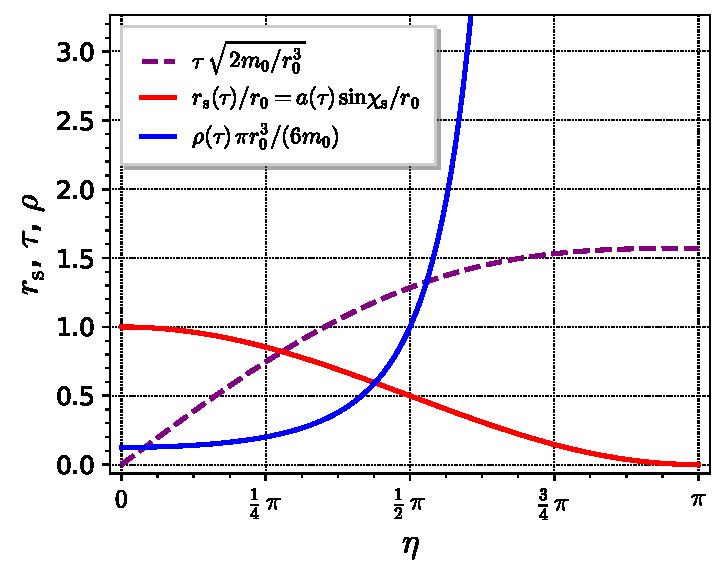
\includegraphics[width=0.48\textwidth]{lem_OS_rs_rho_eta.pdf}\quad
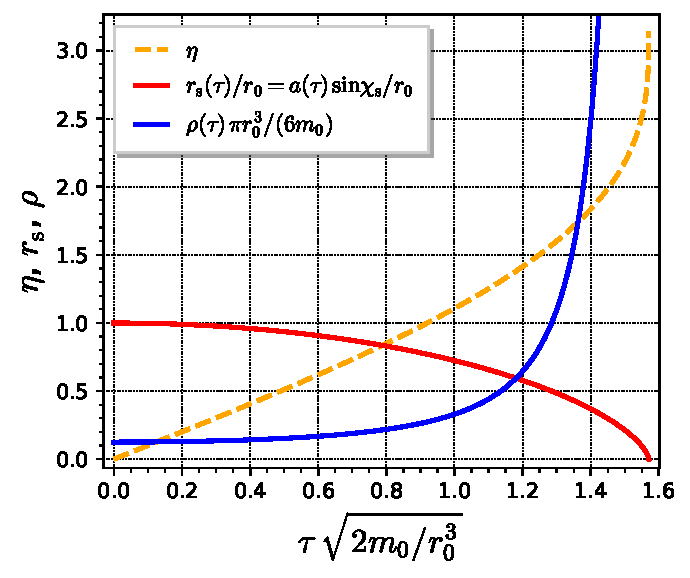
\includegraphics[width=0.45\textwidth]{lem_OS_rs_rho_tau.pdf}
}
\caption[]{\label{f:lem:OS:rs_tho} \footnotesize
Evolution of the areal radius $r_{\rm s}(\tau)$ the collapsing star [Eq.~(\ref{e:lem:OS:evol_star_surf}); red curve] and of the proper matter density
$\rho(\tau)$ [Eq.~(\ref{e:lem:OS:rho_tau}); blue curve] in terms of the conformal time $\eta$ (left)
or the matter proper time $\tau$ (right).  The function $\tau = \tau(\eta)$ is depicted by the purple dashed curve, while its inverse, $\eta = \eta(\tau)$, is depicted by the orange dashed one.
As indicated in the legends, the plot of metric
factor $a(\tau)$ is the same as that of $r_{\rm s}(\tau)$ up to a rescaling
by $\sin\chi_{\rm s}$.
\textsl{[Figures generated by the notebook \ref{s:sam:Oppenheimer_Snyder}]}
}
\end{figure}


The matter density $\rho(\tau,\chi)$ is deduced from Eq.~(\ref{e:lem:LTeqs2}), with the above
values of $m(\chi)$ and $r(\tau,\chi)$. We get a function of $\tau$ only,
via $\eta = \eta(\tau)$ [cf. Eq.~(\ref{e:lem:OS:tau_r_eta})],
which we rewrite as $\rho(\tau)$:
\be \label{e:lem:OS:rho_tau}
  \encadre{  \rho(\tau) = \frac{6 m_0}{\pi r_0^3 (1 + \cos\eta)^3} } .
\ee
% \rho(\tau) = \frac{3 a_0}{8\pi a(\tau)^3}
The independence of $\rho$ from $\chi$ confirms that the choice
(\ref{e:lem:OS:free_func}) leads to a uniform density object, i.e.
a homogeneous star.
Let us stress that the homeogeneity is maintained during all the collapse:
at each instant of matter proper time $\tau$, the density is uniform is all the star.
The function $\rho(\tau)$ is plotted in Fig.~\ref{f:lem:OS:rs_tho}.
\begin{remark}
In view of Eq.~(\ref{e:lem:OS:evol_star_surf}), we may rewrite Eq.~(\ref{e:lem:OS:rho_tau})
as
\be \label{e:lem:OS:rho_m0_r_tau}
    \rho(\tau) = \frac{m_0}{\frac{4}{3}\pi r_{\rm s}(\tau)^3} .
\ee
This formula happens to be identical to that giving the mass density of a uniform ball of mass
$m_0$ and radius $r_{\rm s}(\tau)$ in Newtonian physics (flat spacetime), but there is
no profound physical significance in this coincidence.
\end{remark}

It is instructive to express the initial energy density, $\rho_0 := \rho(\tau=0)$,
in terms of the geometrical energy/mass unit, $m_0^{-2}$, and the compactness
angle $\chi_{\rm s}$ by combining Eqs.~(\ref{e:lem:OS:rho_tau}) and
(\ref{e:lem:OS:sin_chis_m0_r0}):
\be \label{e:lem:OS:rho0}
    \rho_0 = \frac{3 \sin^6\chi_{\rm s}}{32\pi m_0^2} .
\ee

The metric factor $a(\tau,\chi)$, which appears in Eq.~(\ref{e:lem:metric_sync_coord}),
is deduced from Eq.~(\ref{e:lem:a_f_dr}), with $\dert{r}{\chi}$ computed
from expression (\ref{e:lem:OS:tau_r_eta}); as for $\rho$, we get a function of $\tau$
only, which we rewrite as $a(\tau)$:
\be \label{e:lem:OS:a_tau}
   \encadre{ a(\tau) = \frac{a_0}{2} \left( 1 + \cos\eta \right) }.
\ee
We may then rewrite the second equation in (\ref{e:lem:OS:tau_r_eta}) as
$r(\tau,\chi) = a(\tau) \sin\chi$, so that the metric
expression (\ref{e:lem:metric_sync_coord}) inside the star takes the form
\be \label{e:lem:OS:g_interior_tau}
  \encadre{ \w{g} = - \dd\tau^2 + a(\tau)^2 \left[ \dd\chi^2
        + \sin^2\chi \left( \dd\th^2 + \sin^2\th\, \dd\ph^2 \right) \right]  } .
\ee
We recognize a \defin{Friedmann-Lemaître-Robertson-Walker (FLRW) metric}\index{Friedmann-Lemaître-Robertson-Walker metric}\index{FLRW metric} describing a closed universe. This is not so surprising since FLRW metrics are solution of Einstein equations based on the hypothesis of homogeneity of spatial slices (cf. e.g. Chap.~3 of Ref.~\cite{PeterU09}).
We may use $\eta$, instead of $\tau$, as the time coordinate inside the star, thanks to the
relation
\be
    \dd\tau = \frac{a_0}{2} (1 + \cos\eta) \dd\eta ,
\ee
which follows from (\ref{e:lem:OS:tau_r_eta}). We then deduce from Eq.~(\ref{e:lem:OS:g_interior_tau})
that
\be \label{e:lem:OS:g_int}
    \encadre{   \w{g} = \frac{a_0^2}{4} (1 + \cos\eta)^2 \left[ - \dd\eta^2 + \dd\chi^2
        + \sin^2\chi \left( \dd\th^2 + \sin^2\th\, \dd\ph^2 \right) \right] } .
\ee
The term inside square brackets is nothing but the metric $\tilde{\w{g}}$ of the
\emph{Einstein cylinder}\index{Einstein!cylinder} introduced in Sec.~\ref{s:glo:conf_complet_Mink}
[compare Eq.~(\ref{e:glo:tg_Einstein}) with the change of notation $\eta \leftrightarrow \tau$].
Hence, inside the star, the metric $\w{g}$ is conformal to $\w{\tilde{g}}$:
$\w{g} = \Omega^2 \w{\tilde{g}}$,
with the conformal factor $\Omega := a_0/2 (1 + \cos\eta) = a(\tau)$.
For this reason, $\eta$ is called the \defin{conformal time}\index{conformal!time}\index{time!conformal --}.
Note that while $\w{\tilde{g}}$
is a static metric [it obeys Eq.~(\ref{e:sta:static_metric})], $\w{g}$ is not, since
the conformal factor depends on $\eta$.


\begin{figure}
\centerline{
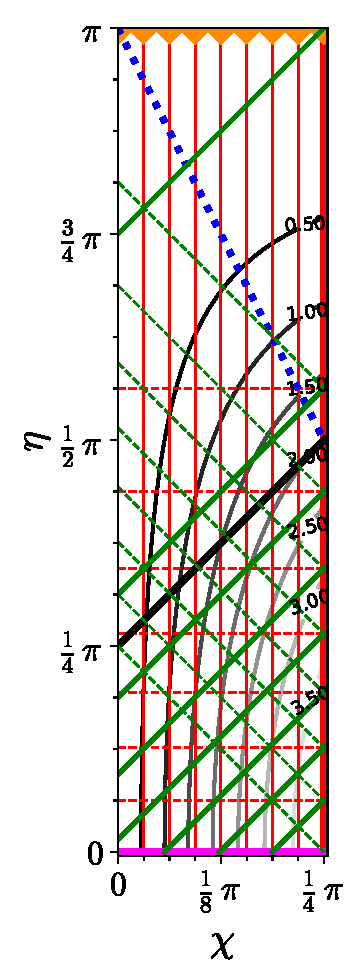
\includegraphics[height=0.55\textheight]{lem_OS_diag_int.pdf}\qquad
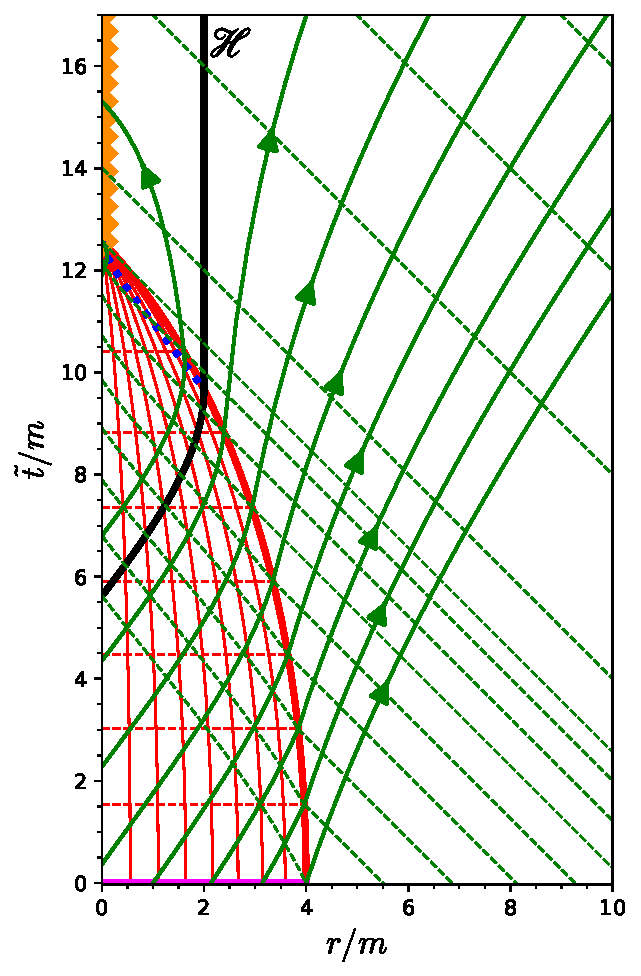
\includegraphics[height=0.6\textheight]{lem_OS_diag_EF.pdf}
}
\caption[]{\label{f:lem:OS:diag_int_EF} \footnotesize
Spacetime diagrams of the Oppenheimer-Snyder collapse
in conformal coordinates $(\eta,\chi)$ (left figure, depicting only the
interior)
and in Eddington-Finkelstein coordinates $(\ti, r)$
(right figure), for an initial compactness $m_0/r_0 = 1/4$, which corresponds to $\chi_{\rm s} = \pi/4$.
In both figures, solid red lines are worldlines of matter particles,
uniformly sampling $[0,\chi_{\rm s}]$ with $\delta\chi=\pi/32$,
while dashed red lines denote isosurfaces of constant matter proper time $\tau$
uniformly sampling $[0,\tau_{\rm end}]$ with $\delta\tau = \tau_{\rm end}/8$.
The thick red line is the star's surface and the thick magenta one is
the star at the initial instant $\tau=0$. The orange zig-zag line marks the
curvature singularity. Solid (resp. dashed) green lines are outgoing (resp. ingoing) radial null geodesics
encountering the star's surface at the above selected values of $\tau$.
The thick black line is the black hole event horizon and the dotted blue line
is the centered inner trapping horizon. In the left figure,
thin solid grey to black lines mark isosurfaces of constant values of the areal radius
$r(\tau,\chi)$ (labelled in units of $m_0$).
\textsl{[Figures generated by the notebook \ref{s:sam:Oppenheimer_Snyder}]}
}
\end{figure}


\begin{figure}
\centerline{
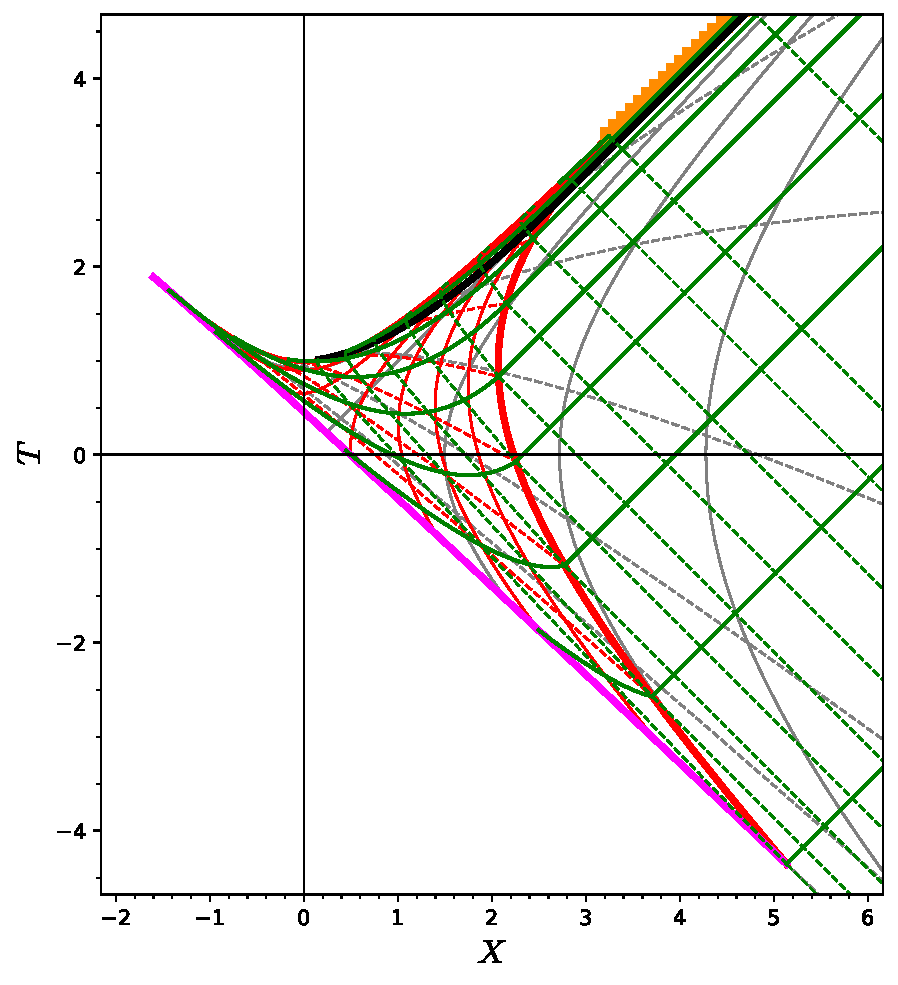
\includegraphics[width=0.55\textwidth]{lem_OS_diag_KS.pdf}\quad
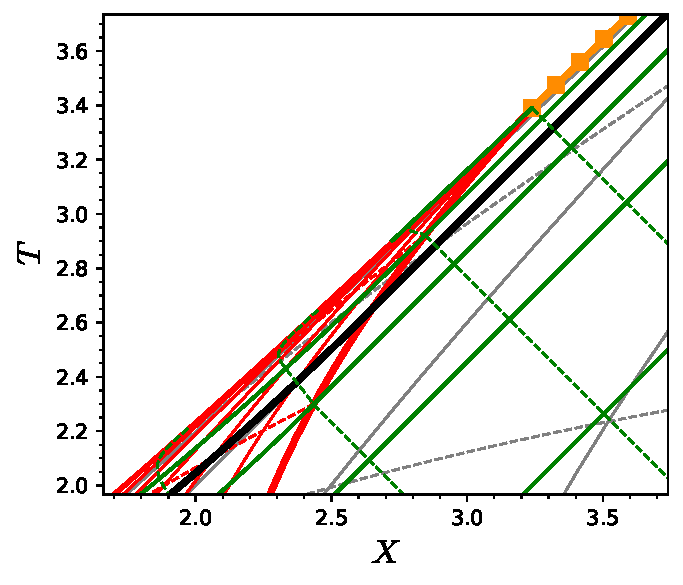
\includegraphics[width=0.45\textwidth]{lem_OS_diag_KS_zoom.pdf}
}
\caption[]{\label{f:lem:OS:diag_KS} \footnotesize
Spacetime diagrams of the Oppenheimer-Snyder collapse
in Kruskal-Szekeres-type coordinates $(T,X)$.
The colored curves are the same as in Fig.~\ref{f:lem:OS:diag_int_EF}.
In particular, the magenta curve represents the star at the start of
the collapse, at $\tau = \tilde{t} = 0$. In addition, solid grey
lines are hypersurfaces of constant $r$, uniformly sampling $[0, 8m_0]$
with $\delta r = m_0$ and dashed lines are hypersurfaces of
constant $\tilde{t}$, uniformly sampling $[0, 16m_0]$ with
$\delta\tilde{t} = 2 m_0$.
The right figure is a zoom on the end of the collapse.
\textsl{[Figures generated by the notebook \ref{s:sam:Oppenheimer_Snyder}]}
}
\end{figure}


On each hypersurface $\eta=\mathrm{const}$ ($\iff \tau = \mathrm{const}$),
the 3-metric induced by
the conformal metric $\w{\tilde{g}}$ is the standard metric of the hypersphere
$\mathbb{S}^3$, expressed in terms of the hyperspherical coordinates $(\chi,\th,\ph)$.
On the whole $\mathbb{S}^3$, $\chi$ ranges from $0$ to $\pi$. Since in the
present case, $\chi \in [0,\chi_{\rm s}]$ [Eq.~(\ref{e:lem:OS:range_chi})],
we may view each constant proper time slice of the interior of the collapsing
star as a piece of $\mathbb{S}^3$, scaled by the factor $a(\tau)$
given by Eq.~(\ref{e:lem:OS:a_tau}).
If one uses the conformal coordinates $(\eta,\chi)$ to draw a 2-dimensional
spacetime diagram of the interior, as in the left part of Fig.~\ref{f:lem:OS:diag_int_EF},
then the radial null geodesics appear as straight lines inclined by $\pm 45^\circ$
with the horizontal, reflecting the Minkowskian part $- \dd\eta^2 + \dd\chi^2$
in the metric (\ref{e:lem:OS:g_int}).

To draw a full spacetime diagram of the collapse, we may extend the ingoing
Eddington-Finkelstein (IEF) coordinates $(\ti,r,\th,\ph)$, used to described the
Schwarschild exterior of the star to the interior region by demanding
that relation (\ref{e:lem:OS:ti_star_surf}), which a priori links $\ti$
to $\eta$ at the stellar surface, holds everywhere in the interior.
As for the IEF coordinate $r$, it is naturally identified with the areal
radius $r(\eta,\chi)$ given by Eq.~(\ref{e:lem:OS:tau_r_eta}).
The resulting spacetime diagram is shown in the right part of Fig.~\ref{f:lem:OS:diag_int_EF}.
In this one, only the ingoing radial null geodesics in the exterior appear
as straight lines, as a consequence of the definition of the IEF coordinates
(cf. Sec.~\ref{s:sch:EF_coord}). The slices of constant proper time $\tau$
(dashed red lines) appear as horizontal line segments by virtue of the above
choice for $\ti$ in the interior. In particular, the star at $\tau = 0$
is depicted by a horizontal magenta segment, as in the $(\eta,\chi)$ diagram
on the left of the figure.


\subsection{Final singularity}

The collapse ends at $\eta = \pi$, since this corresponds to the surface
areal radius $r_{\rm s}(\tau) = 0$ by virtue of Eq.~(\ref{e:lem:OS:evol_star_surf}).
Equation~(\ref{e:lem:OS:tau_r_eta}) shows that this corresponds as well
to $r(\tau,\chi) = 0$ for all
particles inside the star. The matter proper time $\tau$ at the end of the collapse
is given by $\eta=\pi$ in Eq.~(\ref{e:lem:OS:tau_r_eta}):
\be \label{e:lem:OS:tau_end}
   \encadre{ \tau_{\rm end} = \frac{\pi}{2} a_0 = \pi \sqrt{\frac{r_0^3}{8 m_0}}
      = \pi \left( \frac{r_0}{2 m_0} \right)^{3/2} m_0
      = \pi \frac{m_0}{\sin^3\chi_{\rm s}}
      = \sqrt{\frac{3\pi}{32\rho_0}} },
\ee
where the last equality has been obtained by using Eq.~(\ref{e:lem:OS:rho0})
to express $m_0/\sin^3\chi_{\rm s}$ in terms of the initial proper energy density $\rho_0$.
We note that $\tau_{\rm end}$ is a function of $\rho_0$ only.

\begin{remark}
The above formulas for the collapse proper time $\tau_{\rm end}$ are identical
to those giving the collapse time of a spherical ball of dust of mass $m_0$, initial radius
$r_0$ and initial mean mass density $\rho_0=3 m_0/(4\pi r_0^3)$ in Newtonian gravity.
This coincidence arises from the
same cycloidal law for $r_{\rm s}(\tau)$ in both general relativity and Newtonian gravity,
as already discussed in Remark~\ref{r:lem:OS:cycloid} on p.~\pageref{r:lem:OS:cycloid}.
\end{remark}

Similarly, setting $\eta=\pi$ in Eq.~(\ref{e:lem:OS:ti_star_surf}), we get the value
of the IEF coordinate $\ti$ at the end of the collapse:
\be
     \ti_{\rm end} = 2m_0 \left[ \pi \left(1 +  \frac{r_0}{4m_0} \right) \sqrt{\frac{r_0}{2m_0} - 1}
     - \ln \left( \frac{r_0}{2m_0} - 1\right) \right] .
\ee
\begin{example}
For the compactness $m_0/r_0 = 1/4$, which is that considered in Figs.~\ref{f:lem:OS:diag_int_EF}-\ref{f:lem:OS:diag_KS}, the above formulas yield
$\tau_{\rm end} = 2 \sqrt{2} \pi m_0 \simeq 8.89\, m_0$ and
$\ti_{\rm end} = 4 \pi m_0 \simeq 12.57\, m_0$.
\end{example}

Equation~(\ref{e:lem:OS:rho_tau}) with $\eta\to \pi$
immediately yields an infinite proper energy density at the end of the collapse:
\be
    \lim_{\tau\to\tau_{\rm end}} \rho(\tau) = + \infty.
\ee
Since $\rho$ is a measurable quantity (by comoving observers), this signals
some physical singularity.
This corresponds actually to the apparition of a \emph{curvature singularity}
in the part of spacetime covering the interior of the star (cf. the discussion
in Sec.~\ref{s:sch:singularities}).
Indeed, from the interior metric (\ref{e:lem:OS:g_int}), one can
compute\footnote{See the notebook \ref{s:sam:Oppenheimer_Snyder_curvature} for
the computation.} curvature scalars like the Ricci scalar
\be \label{e:lem:OS:Ricci_scal}
    R := R^\mu_{\ \, \mu} = \frac{24}{a_0^2 (1 + \cos\eta)^3} = \frac{6 m_0}{r_{\rm s}(\tau)^3} ,
\ee
the ``square'' of the Ricci tensor
\be \label{e:lem:OS:Ricci_squared}
    R_{\mu\nu} R^{\mu\nu} = \frac{576}{a_0^4 (1 + \cos\eta)^6}
    =  \frac{36 m_0^2}{r_{\rm s}(\tau)^6}
\ee
and the Kretschmann
scalar\index{Kretschmann scalar! of Oppenheimer-Snyder metric} defined by
Eq.~(\ref{e:sch:def_Kretschmann}):
\be \label{e:lem:OS:Kretschmann}
      K := R_{\mu\nu\rho\sigma} R^{\mu\nu\rho\sigma} = \frac{960}{a_0^4 (1 + \cos\eta)^6}
         = \frac{60 m_0^2}{r_{\rm s}(\tau)^6} .
\ee
\begin{remark}
Although the components of the Riemann and Ricci tensors with respect to the
coordinates $(\eta,\chi,\th,\ph)$ depend on $\chi$ (cf. the notebook \ref{s:sam:Oppenheimer_Snyder_curvature}),
the above three scalars are independent
of it, in full agreement with the homogeneity of the stellar interior at each
instant $\eta$.
\end{remark}

It is clear that the above three curvature invariants diverge when $\eta\to \pi$,
or equivalently, when $r_{\rm s}(\tau)\to 0$. Hence a curvature singularity
appears in the stellar interior at the end of the collapse.
It is depicted by the orange zig-zag segment in left spacetime diagram
of Fig.~\ref{f:lem:OS:diag_int_EF}. This singularity is shrinked to the point
$(\ti, r) = (\ti_{\rm end}, 0)$ in the IEF diagram on the right part of the figure,
because $r_{\rm s}(\tau_{\rm end}) = 0$. It is then connected to the
curvature singularity at $r=0$ of Schwarzschild spacetime, depicted as the
vertical orange zig-zag segment.

\begin{remark}
The reader might be puzzled by the Kretschmann scalar (\ref{e:lem:OS:Kretschmann})
being different from that of Schwarzschild spacetime, as given by Eq.~(\ref{e:sch:value_Kretschmann}):
$K_{\rm Schwarz} = 48 m^2/r^6$. Both
have the same $m^2/r^6$ structure but they differ by the numerical prefactor: 60 versus 48.
This actually reflects the discontinuity of the Riemann tensor between the stellar interior
and the Schwarzschild exterior. This discontinuity is enforced on the Ricci part of the Riemann
tensor via the Einstein equation and the uniform density of the star, the latter resulting in
a jump of the energy-momentum tensor $\w{T}$ between the value (\ref{e:lem:T_pressureless})
and zero (vacuum exterior). The difference is even more dramatic on the Ricci scalar
(\ref{e:lem:OS:Ricci_scal})
and the square of the Ricci tensor (\ref{e:lem:OS:Ricci_squared}), since they are
identically zero in the Schwarzschild exterior. In other words, the Einstein equation
implies that the metric tensor of the Oppenheimer-Snyder solution is not $C^2$.
For an actual stellar core, there is a density gradient so that $\rho=0$
at the surface and the metric tensor is $C^2$ (at least).
\end{remark}

\begin{table}
\centerline{
\begin{tabular}{|l|c|c|c|c|}
\hline
& Earth & Sun & white dwarf & neutron star \\[0.5ex]
\hline\hline
$m_0$ $[M_\odot]$& $3 \; 10^{-6}$ & $1$ & $0.6$ & $1.4$ \\[0.5ex]
\hline
$r_0$ $[{\rm km}]$ & $6.37\; 10^3$ & $6.96\; 10^5$ & $8.0\; 10^3$ &  $12$ \\[0.5ex]
\hline
$m_0/r_0$ & $7.0\;10^{-10}$ & $2.1\; 10^{-6}$ & $1.1\; 10^{-4}$ & $0.17$ \\[0.5ex]
\hline
$\chi_{\rm s}$ & $3.7\; 10^{-5}$ & $2.1\; 10^{-3}$ & $1.5\; 10^{-2}$ & $0.63$ \\[0.5ex]
\hline
$\rho_0$ $[{\rm kg\, m}^{-3}]$ & $5.5\; 10^3$ & $1.4\; 10^3$ & $5.6\; 10^8$ & $3.8\; 10^{17}$ \\[0.5ex]
\hline
$\tau_{\rm end}$ & $14\; {\rm min}\; 55\; {\rm s}$ & $29\; {\rm min}\; 30\; {\rm s}$ &
$2.82\; {\rm s}$ & $0.107\; {\rm ms}$  \\[0.5ex]
\hline
$\tau_{\rm hb}$ & $14\; {\rm min}\; 55\; {\rm s}$ & $29\; {\rm min}\; 30\; {\rm s}$ &
$2.82\; {\rm s}$ & $0.075\; {\rm ms}$  \\[0.5ex]
\hline
$\tau_{\rm end} - \tau_{\rm hb}$ & $6.6\; 10^{-11}\; {\rm s}$ & $22\; \mu{\rm s}$
& $13\; \mu{\rm s}$ & $22\; \mu{\rm s}$ \\[0.5ex]
\hline
$\tau_{\rm end} - \tau_*$ & $2.0\; 10^{-11}\; {\rm s}$ & $6.6\; \mu{\rm s}$
& $3.9\; \mu{\rm s}$ & $10.4\; \mu{\rm s}$ \\[0.5ex]
\hline
$\rho_{\rm hb}$ $[{\rm kg\, m}^{-3}]$ & $1.8\; 10^{29}$ & $1.8\; 10^{18}$
& $4.5\; 10^{18}$ & $1.4\; 10^{18}$ \\[0.5ex]
\hline
\end{tabular}
}
\caption[]{\label{t:lem:OS:num} \footnotesize
Numerical values for the gravitational collapse of various astrophysical bodies,
assuming that all forces counterbalancing gravitation suddenly disappear
at the proper time $\tau=0$.
$m_0$ is the gravitational mass (constant during the collapse),
$r_0$ is the initial areal radius, $m_0/r_0$ is the initial compactness,
$\chi_{\rm s}$ is the (constant) value of the hyperspherical angle $\chi$ at the surface
of the body [Eq.~(\ref{e:lem:OS:chis_m0_r0})], $\rho_0$ is the initial
proper energy density, assuming that the body is homogeneous
[Eq.~(\ref{e:lem:OS:rho_m0_r_tau}) with $\tau=0$, or Eq.~(\ref{e:lem:OS:rho0})],
$\tau_{\rm end}$ is the proper time at the end of the collapse, when the
central singularity appears [Eq.~(\ref{e:lem:OS:tau_end})],
$\tau_{\rm hb}$ is the proper time of the event horizon birth at the center
of the body [Eq.~(\ref{e:lem:OS:tau_hb})],
$\tau_*$ is the proper time when the event horizon encounters
the infalling surface [Eq.~(\ref{e:lem:OS:tau_star})]
and $\rho_{\rm hb}$ is the proper energy density
at $\tau=\tau_{\rm hb}$, i.e. when the black hole forms [Eq.~(\ref{e:lem:OS:rho_hb})].
}
\end{table}



\subsection{Black hole formation}

Since the surface areal radius $r_{\rm s}(\tau)$ is a monotonically decreasing function
of $\tau$ (cf. Fig.~\ref{f:lem:OS:rs_tho}), there exists a unique value $\tau_*$ of
$\tau$ for which $r_{\rm s}(\tau_*) = 2 m_0$. For $\tau>\tau_*$, $r_{\rm s}(\tau) < 2 m_0$
and the exterior
Schwarzschild spacetime contains a black hole event horizon $\Hor$, located
at $r=2m_0$ in IEF coordinates (the vertical black segment in Fig.~\ref{f:lem:OS:diag_int_EF}).
The value of $\tau_*$ is determined through the corresponding
conformal time $\eta_*$ via Eq.~(\ref{e:lem:OS:evol_star_surf}):
\[
    \frac{r_0}{2} (1 + \cos\eta_*) = 2 m_0 \iff
    \cos\eta_* = 4\frac{m_0}{r_0} - 1 = 2 \sin^2\chi_{\rm s} - 1 = - \cos(2\chi_{\rm s}) ,
\]
where use has been made of Eq.~(\ref{e:lem:OS:sin_chis_m0_r0}). Given that $0<\eta_*<\pi$
and $0<\chi_{\rm s} < \pi/2$, the solution is
\be \label{e:lem:OS:eta_star}
    \eta_* = \pi - 2 \chi_{\rm s} .
\ee
Equation~(\ref{e:lem:OS:evol_star_surf}) yields then
\be \label{e:lem:OS:tau_star}
    \tau_* = \frac{\pi - 2 \chi_{\rm s} + \sin(2\chi_{\rm s})}{\sin^3\chi_{\rm s}} m_0
     =  \left( 1 - \frac{2\chi_{\rm s} - \sin(2\chi_{\rm s})}{\pi} \right) \tau_{\rm end} .
\ee

\begin{example}
For the compactness $1/4$ considered in
Figs.~\ref{f:lem:OS:diag_int_EF}-\ref{f:lem:OS:diag_KS}, one has $\chi_{\rm s}=\pi/4$,
so that $\eta_* = \pi/2$ and
$\tau_* = \sqrt{2}(\pi + 2) m_0 \simeq 7.27 \, m_0 \simeq 0.82 \, \tau_{\rm end}$.
\end{example}

For $\tau < \tau_*$, one has $r_{\rm s}(\tau) > 2 m_0$ and the event horizon
must be located inside the collapsing star. To determine it,
let us consider the outgoing radial null geodesics, which are drawn as solid green curves
in Fig.~\ref{f:lem:OS:diag_int_EF}. In view of the metric (\ref{e:lem:OS:g_int}),
the equation of such a geodesic is very simple in terms of
the coordinates $(\eta,\chi)$: $\eta = \chi - \chi_{\rm s} + \eta_{\rm s}$, where
the constant $\eta_{\rm s}$ is the value of $\eta$ when the geodesic
reaches the surface of the star ($\chi = \chi_{\rm s}$). Radial null geodesics
for which $\eta_{\rm s} < \eta_*$ emerge out of the star in
a part of Schwarschild spacetime where $r > 2 m_0$, so that they can espace
to infinity. On the contrary, geodesics having $\eta_{\rm s} > \eta_*$ emerge in the
black hole region of Schwarzschild spacetime; they are thus trapped and
eventually end on the curvature singularity at $r=0$. The event horizon
is generated by the null radial geodesics of the limiting case: $\eta_{\rm s} = \eta_*$.
Hence, inside the star, the equation of the black hole event horizon $\Hor$
is $\eta = \chi - \chi_{\rm s} + \eta_*$. Given the value (\ref{e:lem:OS:eta_star}) for
$\eta_*$, we get
\be \label{e:lem:OS:Hor_eta_chi}
    \Hor:\qquad \eta = \chi + \pi - 3 \chi_{\rm s} .
\ee
For a fixed value of $(\th,\ph)$, this is the equation of a straight line segment
inclined by $+45^\circ$ with
respect to the horizontal.

The equation of $\Hor$ in terms of the internal IEF coordinate is obtained in parametric
form, with parameter $\chi\in[0,\chi_{\rm s}]$ by substituting (\ref{e:lem:OS:Hor_eta_chi})
for $\eta$ in Eq.~(\ref{e:lem:OS:ti_star_surf}) providing $\ti$ and in
Eq.~(\ref{e:lem:OS:tau_r_eta}) providing $r$. One obtains then a curved segment
in the $(\ti, r)$ plane, which
is drawn in black in Fig.~\ref{f:lem:OS:diag_int_EF}, right.

In view of Eq.~(\ref{e:lem:OS:Hor_eta_chi}), we may say that
\begin{greybox}
The event horizon $\Hor$ appears at the center of the star ($\chi=0$)
at the conformal time
\be \label{e:lem:OS:eta_hb}
    \eta_{\rm hb} = \pi - 3 \chi_{\rm s}
\ee
or equivalently at the matter proper time
\be \label{e:lem:OS:tau_hb}
  \tau_{\rm hb} = \frac{\pi - 3 \chi_{\rm s} + \sin(3\chi_{\rm s})}{\sin^3\chi_{\rm s}} m_0
     =  \left( 1 - \frac{3\chi_{\rm s} - \sin(3\chi_{\rm s})}{\pi} \right) \tau_{\rm end} ,
\ee
the label `hb' standing for ``horizon birth''.
The horizon then expands according to Eq.~(\ref{e:lem:OS:Hor_eta_chi}) until it reaches the surface
of the star ($\chi=\chi_{\rm s}$) at $\eta = \eta_* = \pi - 2 \chi_{\rm s}$
or $\tau = \tau_*$ given by Eq.~(\ref{e:lem:OS:tau_star}).
\end{greybox}

\begin{example}
Continuing with the example $m_0/r_0=1/4 \iff \chi_{\rm s}=\pi/4$,
we get $\eta_{\rm hb} = \pi/4$, which corresponds to the origin of the
black straight segment drawn in Fig.~\ref{f:lem:OS:diag_int_EF}, left.
Equation~(\ref{e:lem:OS:tau_hb}) gives
$\tau_{\rm hb} = (2 + \pi/\sqrt{2}) m_0 \simeq 4.22 \, m_0 \simeq 0.48 \, \tau_{\rm end}$.
\end{example}

\begin{figure}
\centerline{
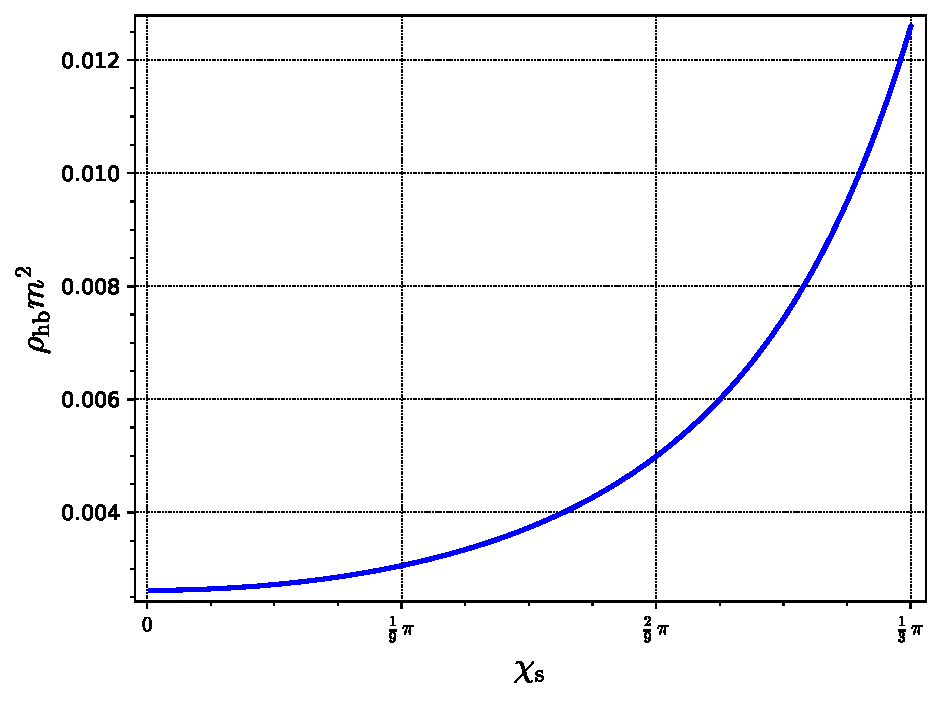
\includegraphics[height=0.35\textheight]{lem_OS_rho_hb.pdf}
}
\caption[]{\label{f:lem:OS:rho_hb} \footnotesize
Proper energy density $\rho_{\rm hb}$ at the instant of the black hole
formation at the center of the star, in units of $m_0^{-2}$,
as a function of the initial compactness angle $\chi_{\rm s}$.
\textsl{[Figure generated by the notebook \ref{s:sam:Oppenheimer_Snyder}]}
}
\end{figure}


The matter proper energy density at the horizon birth,
i.e. at $\tau = \tau_{\rm hb}$, is obtained by substituting (\ref{e:lem:OS:eta_hb})
for $\eta$ into Eq.~(\ref{e:lem:OS:rho_tau}); using the identity (\ref{e:lem:OS:sin_chis_m0_r0})
to express $m_0^3/r_0^3$ in terms of $\chi_{\rm s}$, we get
\be \label{e:lem:OS:rho_hb}
    \rho_{\rm hb} := \rho(\tau_{\rm hb}) = \frac{3}{4\pi m_0^2} \frac{\sin^6\chi_{\rm s}}{(1 - \cos(3\chi_{\rm s}))^3} .
\ee
It is instructive to take the limit of small initial compactness $m_0/r_0 \ll 1$,
which corresponds to $\chi_{\rm s} \ll 1$ by virtue of relation~(\ref{e:lem:OS:chis_m0_r0}):
\be \label{e:lem:OS:rho_hb_small_compact}
    \rho_{\rm hb}\simeq \frac{2}{243\pi m_0^2} \left( 1 + \frac{5}{4} \chi_{\rm s}^2 \right)
    + O(\chi_{\rm s}^4) .
\ee
We deduce from Eqs.~(\ref{e:lem:OS:rho_hb})-(\ref{e:lem:OS:rho_hb_small_compact}) that
\be
    \lim_{\chi_{\rm s}\to 0} \rho_{\rm hb} = \frac{2}{243\pi m_0^2}
    \simeq 2.62\; 10^{-3} m_0^{-2}
    \quad\mbox{and}\quad
    \lim_{\chi_{\rm s}\to \pi/2}  \rho_{\rm hb} = \frac{3}{4\pi m_0^2}
    \simeq 0.239\, m_0^{-2}.
\ee
Between these two limits, $\rho_{\rm hb}$ has a monotonic behavior, as shown in
Fig.~\ref{f:lem:OS:rho_hb}. In particular, we have
\be
    \rho_{\rm hb} < \frac{1}{4 m_0^2} .
\ee
Hence
\begin{greybox}
By selecting a sufficiently large mass $m_0$, the matter proper energy density
when the black hole region forms at the center of the collapsing star
can be made arbitrarily small.
\end{greybox}
\begin{example}
Let us a consider the density of water: $\rho_{\rm hb} = 10^3 \; {\rm kg\, m}^{-3}$.
By restoring the $G$'s and the $c$'s, the density $m_0^{-2}$ becomes
$c^6/G^3 m_0^{-2}$.  We get then $m_0 \simeq 4\; 10^7 M_\odot$ for small initial compactness
($\chi_{\rm s} \ll 1$)
and $m_0 \simeq 4\; 10^8 M_\odot$ for large initial compactness
($\chi_{\rm s} \sim \pi/2$).
\end{example}



\subsection{Trapped surfaces}

















